\chapter{Migración}


\section{Introducción}
La Extensión de Implementación y Migración agrega conceptos para respaldar la migración de arquitecturas empresariales, facilitando asi procesos de identifiacion de oportunidades, soluciones y planificación de la misma. Esta fase incluye conceptos para modelar programas y proyectos de implementación para respaldar el programa, la cartera y la gestión de proyectos, y un concepto de “Plateu” para respaldar la planificación de la migración. Se desbriben a continuacion estos conceptos clave para otorgar al lector una mirada mas acertada de este. 
Una \textit{Platea} está vinculada a una arquitectura que es válida durante un cierto lapso de tiempo. Para indicar qué partes de la arquitectura pertenecen a una cierta Platea, una Platea puede agregar cualquiera de los conceptos del núcleo de ArchiMate.
Una \textit{brecha}está asociada con los conceptos básicos que son únicos en una de las Platea conectadas por la brecha; es decir, los conceptos centrales que conforman la diferencia entre estas Platea.
Un \textit{libreable} puede realizar, entre otros, la implementación de una arquitectura o una parte de una arquitectura. Por lo tanto, cualquiera de los conceptos del núcleo de ArchiMate puede vincularse a un entregable por medio de una relación de realización. Al igual que la mayoría de los conceptos básicos, una ubicación puede asignarse a un paquete de trabajo o entregable. Las relaciones más débiles también se pueden definir. Por ejemplo, la relación de asociación puede ser
utilizado para mostrar que ciertas partes de la arquitectura se ven afectadas de algún modo por ciertos paquetes de trabajo.
Estrictamente hablando, las relaciones entre los conceptos de implementación y migración y los conceptos de motivación son relaciones indirectas; por ejemplo, un entregable realiza un requisito u objetivo a través de la realización de un elemento central de ArchiMate (por ejemplo, un componente de aplicación, proceso comercial o servicio). Sin embargo, sigue siendo útil hacer explícitas estas relaciones, para mostrar directamente que se necesita un entregable para cumplir ciertos requisitos y objetivos.
Además, las metas y los requisitos se pueden asociar con cierta Platea; por ejemplo, ciertos requisitos solo pueden ser aplicables a la arquitectura de destino, mientras que otros pueden aplicarse a una determinada arquitectura de transición. Esto se puede modelar por medio de la relación de agregación.


\section{Punto de Vista de Proyecto}
\subsection{Descripción}
El punto de vista de un proyecto se usa principalmente para modelar la gestión del cambio de arquitectura. La "arquitectura" del proceso de migración desde una situación anterior (arquitectura empresarial actual) a una nueva situación deseada (arquitectura empresarial estatal de destino)  este cambio tiene consecuencias siginificativas en la estrategia de crecimiento a medio y largo plazo y en el proceso posterior de toma de decisiones. 
Algunos de los problemas que deben tener en cuenta los modelos diseñados en este punto de vista son:
\begin{itemize}
	\item Desarrollar una arquitectura empresarial completamente desarrollada en toda la organización es una tarea que puede requerir varios años.
	\item Todos los sistemas y servicios deben permanecer operativos independientemente de todas las modificaciones y cambios de la arquitectura empresarial durante el proceso de cambio.
	\item El proceso de cambio puede tener que lidiar con estándares de tecnología inmadura.
	\item El cambio tiene serias consecuencias para el personal, la cultura, la forma de trabajar y la organización.
\end{itemize}
Además de estos , existen otros aspectos que podrían limitar el proceso de transformación. 

\subsubsection{Metamodelo}
\begin{figure}[h]
	\centering
	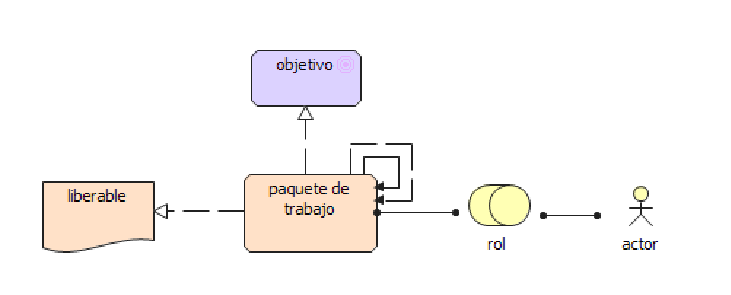
\includegraphics[width=1.0\textwidth]{imagenes/Metamodelos/Migracion/meta_Proyecto.pdf}
	\caption{Metamodelo: Punto de Vista de Proyecto.}
	\label{fig:gap_analysis}
\end{figure}

\subsubsection{Caso de Estudio}
De acuerdo al objetivo fundamental de la organización se asocian dos roles que intervienen en el cumplimiento de este, el Operario, que a su vez se expresa en los actores Cajero y Vigilante. Y, por otro lado, el rol de cliente que es desempeñado por el grupo de ciclistas que hacen uso del servicio de parqueo. Estos roles interactúan directamente con el sistema que se pretende desarrollar con el fin de llevar a cabo el objetivo del sistema.
\\
\\
\\
\\
\\
\\
\\

\begin{figure}[h]
	\centering
	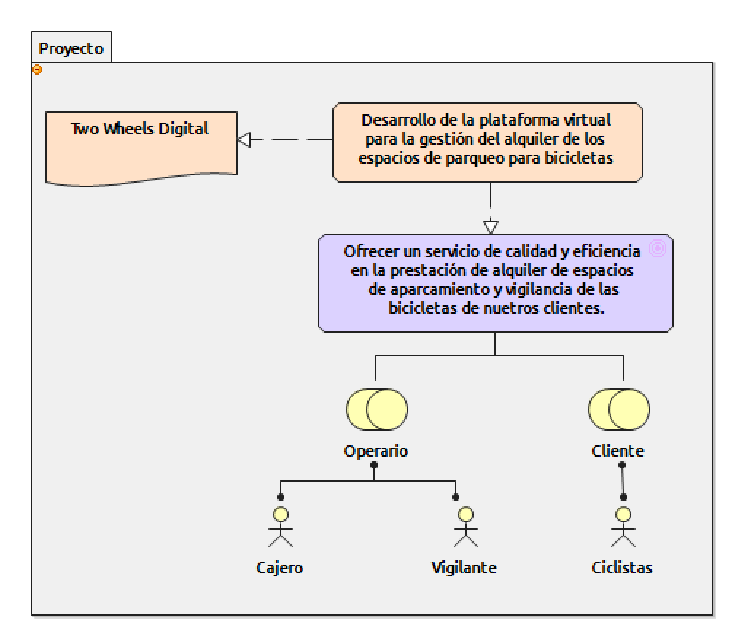
\includegraphics[width=0.8\textwidth]{imagenes/Caso_Estudio/Migracion/Proyecto.PDF}
	\caption{Caso de estudio: Punto de Vista de Proyecto.}
	\label{fig:gap_analysis}
\end{figure}

\section{Punto de Vista de Migración}
\subsection{Descripción}
El punto de vista de migración implica modelos y conceptos que se pueden usar para especificar la transición de una arquitectura existente a una arquitectura deseada. Dado que los conceptos de Platea y brecha se han presentado descrito en esta seccion ampliamnete porcederemos directamente a visualizar el metamodelo y el caso de estudio.

\subsubsection{Metamodelo}
\begin{figure}[h]
	\centering
	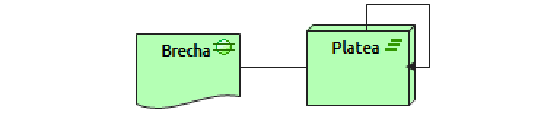
\includegraphics[width=1.0\textwidth]{imagenes/Metamodelos/Migracion/meta_Migracion.pdf}
	\caption{Metamodelo: Punto de Vista de Migración}
	\label{fig:gap_analysis}
\end{figure}

\subsubsection{Caso de Estudio}
Teniendo en cuenta el objetivo del sistema a desarrollar, se busca automatizar los procesos de asignación de espacios de parqueo a ciclistas permitiendo a la empresa poseer un sistema que gestione sus recursos físicos, realizando peticiones sobre la información que se ha almacenado por medio de la herramienta de software como lo es Two Wheels Digital.

\begin{figure}[h]
	\centering
	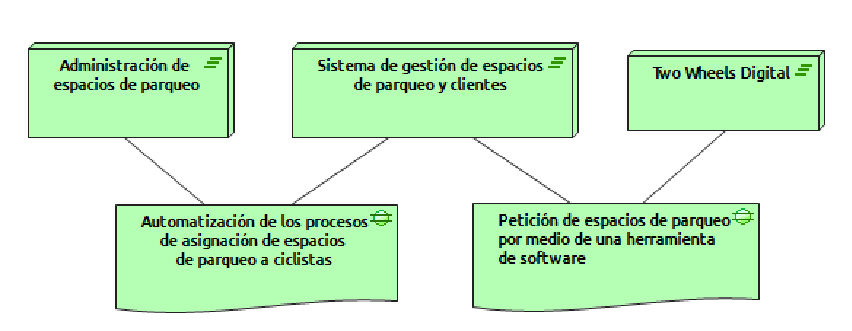
\includegraphics[width=1.0\textwidth]{imagenes/Caso_Estudio/Migracion/Migracion.PDF}
	\caption{Caso de estudio: Punto de Vista de Migración.}
	\label{fig:gap_analysis}
\end{figure}

\section{Punto de Vista de Migración e Implementación}

\subsection{Descripción}
El punto de vista de implementación y migración se usa para relacionar programas y proyectos con las partes de la arquitectura que implementan. Esta vista permite modelar el alcance de los programas, proyectos y ctividades de proyectos en términos de las Plateas que se realizan o la arquitectura en elementos individuales que se ven afectados, además la forma en que los elementos se ven afectados puede ser indicada anotando las relaciones.
Además  de esto es adecuado para relacionar objetivos comerciales (y requisitos) a través de programas y proyectos a (partes de) la arquitectura. Por ejemplo, esto permite analizar la superposición potencial entre las actividades del proyecto o analizar la coherencia entre las restricciones y dependencias del proyecto entre plateas o elementos de arquitectura.

\subsubsection{Metamodelo}
\begin{figure}[h]
	\centering
	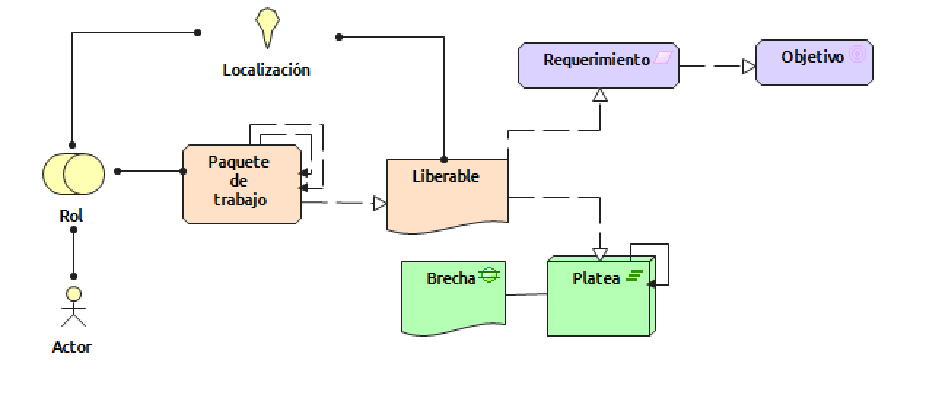
\includegraphics[width=1.0\textwidth]{imagenes/Metamodelos/Migracion/meta_Migracion_implementacion.pdf}
	\caption{Metamodelo: Punto de Vista de Migración e Implementación.}
	\label{fig:gap_analysis}
\end{figure}

\subsubsection{Caso de Estudio}
Este es el resumen de los puntos de vista anteriormente tratados, que son los del proyecto y migración. En este se plantea la visión final de lo que se quiere realizar a través de la arquitectura generada desde las anteriores capas manejadas, y de esta manera delimitar su alcance como proyecto.

\begin{figure}[h]
	\centering
	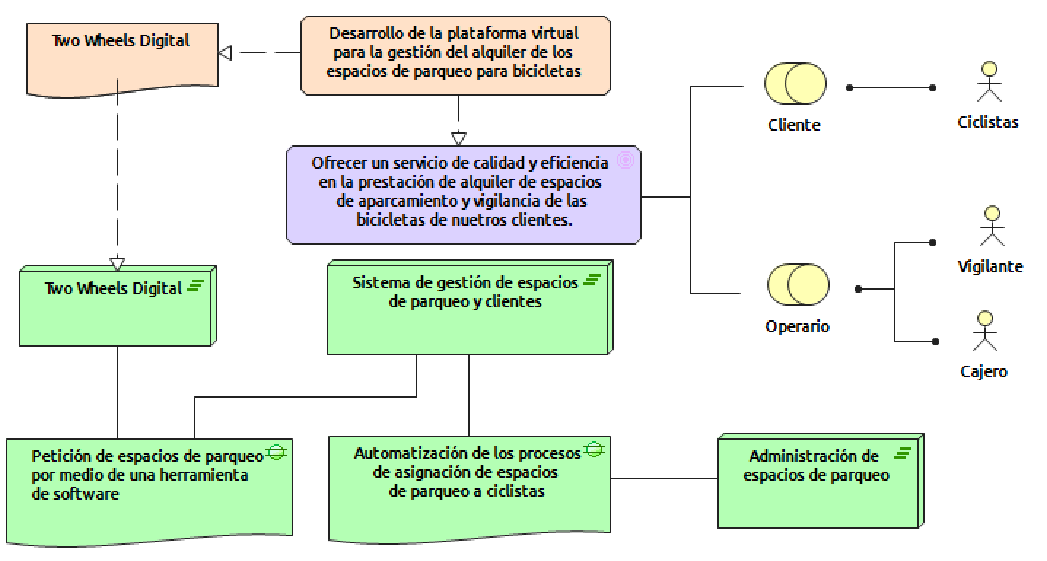
\includegraphics[width=1.0\textwidth]{imagenes/Caso_Estudio/Migracion/Migracion_Implementacion.PDF}
	\caption{Caso de estudio: Punto de Vista de Migración e Implementación.}
	\label{fig:gap_analysis}
\end{figure}

